\documentclass[11pt,a4paper]{report}
\usepackage[utf8]{inputenc}
\usepackage[french]{babel}
\usepackage[T1]{fontenc}
\usepackage{amsmath}
\usepackage{amsfonts}
\usepackage{amssymb}
\usepackage{xcolor}
\usepackage{gensymb}

\usepackage{geometry}
\geometry{hmargin=2.5cm,vmargin=1.5cm}
\usepackage{wasysym}
\usepackage{graphicx}

\author{Mathieu Sarrat}
\title{LC12 - Corps purs et mélanges binaires}

\makeatletter
\renewcommand{\thesection}{\@arabic\c@section}
\makeatother

\begin{document}
\maketitle

\section*{Niveau}
\begin{itemize}
	\item PSI
\end{itemize}

\section*{Pré-requis}
\begin{itemize}
	\item Solides cristallins.
	\item Principes de la Thermodynamique.
\end{itemize}

\section*{Matériel}

\begin{itemize}
	\item acide acétique glacial (pur);
	\item pissette d'acétone pour nettoyer la verrerie;
	\item glace en bonne quantité;
	\item Gros sel (500 g) pour faire un bain glace + sel (permet de descendre plus bas que 0);
	\item Freezer pour le mélange eau sel;
	\item Petit vase Dewar;
	\item Tubes à essais larges;
	\item Tige pour agiter;
	\item Thermomètre classique;
	\item 1 capteur de température Eurosmart, 
		carte d'acquisition et ordinateur portable avec Latis Pro;
\end{itemize}

\section*{Recommandations}
\begin{itemize}
	\item si on ne dispose comme source froide que du mélange glace/eau à 0$\degree$C, ne mettre que 5 gouttes d'eau dans 10 mL d'acide acétique glacial, pour avoir un point de fusion suffisamment éloigné de 0$\degree$C (et ainsi mieux voir la rupture de pente, le refroidissement étant d'autant plus lent que l'écart de température est faible entre le bain de glace et le système qu'on refroidit.
\end{itemize}

\newpage
\section*{Introduction}

Dans notre expérience quotidienne, on sait que l'eau gèle à $0\degree$C à pression atmosphérique. En hiver, dans les régions montagneuses, on met du sel sur les routes pour empêcher la formation de verglas lorsqu'il fait froid. Pourquoi mélanger du sel à de l'eau ? Lorsqu'on fait une soudure étain/plomb, on porte le métal à $183\degree$C et il fond : or, à pression ambiante, l'étain fond à $232\degree$C et le plomb à $327\degree$C. Le mélange des deux métaux semble abaisser la température de fusion.\\

Un corps pur est un système thermodynamique ne comportant qu'une seule espèce chimique, à la différence d'un mélange qui en comporte plusieurs. Le comportement d'un mélange diffère notablement de celui d'un corps pur pour tout ce qui relève des changements d'état, et la fusion ne fait pas exception. L'objectif de cette leçon est de mettre en évidence puis de modéliser ces différences de comportement.

\section{Changement d'état d'un corps pur}

\subsection{Potentiel chimique d'un corps pur}

Jusqu'à présent, nous n'avons travaillé qu'avec des systèmes isolés ou fermés en thermodynamique. Raisonnons avec comme système un corps pur, \textbf{dont la quantité de matière $n$ peut varier} : on parle de \textbf{système ouvert}. Le chimiste \textbf{contrôle en général température et pression} : l'\textbf{enthalpie libre} $G(T,p)$ est le potentiel thermodynamique tout indiqué. Puisque $G$ est extensive et que la quantité de matière peut varier, $G$ dépend donc aussi $n$, variable indépendante de $T$ et $p$ :
\begin{equation}
	dG = \left(\frac{\partial G}{\partial T}\right)_{p,n} dT  
	+  \left(\frac{\partial G}{\partial p}\right)_{T,n} dp  
	+  \left(\frac{\partial G}{\partial n}\right)_{T,p} dn.
\end{equation}
On définit le \textbf{potentiel chimique du corps pur} comme
\begin{equation}
	\mu^*(T,p) \equiv \left(\frac{\partial G}{\partial n}\right)_{T,p},
\end{equation}
d'où pour l'évolution d'un corps pur système ouvert à température et pression constantes
\begin{equation}
	\boxed{dG = \mu^* dn}.\\
\end{equation}

Puisque G est extensive,
\begin{equation}
	G(T,p,n) = n G_m(T,p)
\end{equation}
où $G_m$, l'enthalpie libre molaire, variable intensive qui ne dépend donc plus que de $T$ et de $p$. Si on différencie par rapport à $n$, 
\begin{equation}
	dG = G_m(T,p) dn \quad\text{d'où}\quad
	G_m \equiv \mu^*(T,p).
\end{equation}
\textbf{L'enthalpie libre molaire coïncide avec le potentiel chimique.}\\

Le potentiel chimique est une grandeur intensive jouant un rôle analogue à la température ou à la pression du point de vue de la thermodynamique. Entre deux systèmes :
\begin{itemize}
	\item une différence de $T$ induit des échanges thermiques,
	\item une différence de $p$ induit des échanges de volume,
	\item une différence de $\mu^*$ induit des échanges de matière.\\
\end{itemize}

Ces échanges de matière peuvent avoir lieu :
\begin{itemize}
	\item \textbf{entre deux phases, lors d'un changement d'état},
	\item entre espèces chimiques, lorsqu'il y a réaction.\\
\end{itemize}
Le cas des réactions chimiques sera développé dans une leçon ultérieure. On se limite dans cette leçon au cas des changements d'état.

%\subsection{Influence de la pression et de la température}
%
%Nous cherchons le comportement de $\mu^*$ en fonction de $T$ et $p$, paramètres contrôlés expérimentalement. 
%
%\begin{itemize}
%	\item \textbf{D'une part,} G est extensive, donc
%	\begin{equation}
%		G(T,p,n) = n G_m(T,p)
%	\end{equation}
%	où $G_m$, l'enthalpie libre molaire, variable intensive, ne dépend nécessairement 
%	plus que de $T$ et de $p$. Par conséquent
%	\begin{equation}
%		G_m = \left(\frac{\partial G}{\partial n}\right)_{T,p} = \mu^*(T,p).
%	\end{equation}
%	L'enthalpie libre molaire coïncide avec le potentiel chimique.\\
%	
%	\item \textbf{D'autre part :} relations de Maxwell
%	\begin{equation}
%		\left(\frac{\partial \mu^*}{\partial T}\right)_p = 
%		-\left(\frac{\partial S}{\partial n}\right)_{T,p} = -S_m 
%		\quad\text{et}\quad 
%		\left(\frac{\partial \mu^*}{\partial p}\right)_T 
%		= \left(\frac{\partial V}{\partial n}\right)_{T,p} = V_m 	
%	\end{equation}
%	où
%	\begin{equation}
%		S_m \equiv \frac{S}{n}\quad\text{et}\quad V_m \equiv \frac{V}{n}
%	\end{equation}
%	par extensivité de $S$ et $V$, désignent l'entropie et le volume molaires.\\
%	
%	\item \textbf{Il en résulte que}
%	\begin{equation}
%		d\mu^* = -S_m dT + V_m dp.\\
%	\end{equation}
%	
%	\begin{itemize}
%		\item l'entropie molaire dépend fortement de $T$, l'effet de la température sur 
%		le potentiel chimique d'une espèce est donc à considérer.\\
%		
%		\item le volume molaire $V_m$ varie peu pour les phases condensées
%		\begin{equation}
%			V_m = \frac{M}{\rho},
%		\end{equation}		 
%		où $M$ est la masse molaire et $\rho$ la masse volumique. On négligera l'influence de 
%		la pression sur le potentiel chimique d'un liquide ou d'un solide.\\ 
%		
%		\item \textbf{On ne peut pas négliger cette dépendance pour un gaz.} 
%		Par exemple, pour un gaz parfait
%		\begin{equation}
%			V_m = \frac{RT}{p}.
%		\end{equation}
%		Intégrer par rapport à $p$, entre $p$ et la pression standard $p^\circ$, utilisant la 					seconde relation de Maxwell
%		\begin{equation}
%			\mu^*(T,p) = \mu^*(T,p^\circ) 
%			+ RT\text{ln}\left(\frac{p}{p^\circ}\right).\\
%		\end{equation}
%	\end{itemize}
%	
%	\item Ces différences de comportement nous montrent que \textbf{le potentiel chimique d'un corps 	pur dépend de son état physique et donc de la phase $\phi$ dans laquelle il se trouve} : solide, 	liquide, gazeux, en solution etc...
%	\begin{equation}
%		\mu^*(T,p) = \mu^{*,\phi}(T,p).\\
%	\end{equation}
%\end{itemize}
%	
%\textit{Remarque : si $G_m$ coïncide avec $\mu^*$ pour un corps pur, il n'en va pas de même avec 
%$U_m$, $F_m$ ou $H_m$ qui dépendent explicitement de variables extensives (l'entropie ou le volume). Donc
%\begin{equation}
%	\mu^*=\left(\frac{\partial U}{\partial n}\right)_{S,V}\neq U_m\equiv\frac{U}{n}.
%\end{equation}}
%On omettra tantôt le $*$, tantôt le $\phi$ lorsqu'il n'y aura pas d'ambiguïté possible, pour alléger les notations.

\subsection{Équilibre d'un corps pur sous plusieurs phases}

On va maintenant appliquer la notion de potentiel chimique à la description des changements d'état d'un corps pur. Considérons comme système fermé une quantité de matière d'eau pure $n$, présente sous deux phases, par exemple liquide et solide, contenant chacune $n^l$ et $n^s$ moles d'eau. On modélise cette transformation par l'équation \textcolor{red}{\textbf{(faire un schéma et un tableau d'avancement)}}
\begin{equation}
	\text{H}_2\text{O}_\text{(l)} \rightleftarrows \text{H}_2\text{O}_\text{(s)} 
\end{equation}
et on a $n = n^l + n^s \quad\text{par conservation de la matière}$.\\
	
\textbf{En vertu du Second Principe}, à $T$ et $p$ fixées, égales à $T_\text{ext}$ et $p_\text{ext}$, un système évolue spontanément en minimisant $G$, donc selon :
\begin{equation}
	dG < 0.
\end{equation}

Par extensivité de $G$ :
\begin{equation}
	G = G^\alpha + G^\beta = n^l \mu^{*,l} + n^s \mu^{*,s},
\end{equation}
et $d\xi = -dn^l = dn^s$  d'où
\begin{equation}
	\boxed{dG = \left(\mu^{*,s} - \mu^{*,l} \right) d\xi < 0}.
\end{equation}
Si $\mu^{*,s} < \mu^{*,l}$, $d\xi > 0$ : des molécules passent de la phase liquide vers la phase solide. Changer de phase permet au système d'atteindre un état plus stable thermodynamiquement. Le transfert de matière entre phases se fait \textbf{dans le sens des potentiels chimiques décroissants}.\\

Pour qu'il y ait équilibre entre l'eau liquide et la glace il faut que l'enthalpie libre du système (eau $+$ glace) soit minimale pour un couple $(T,p)$ donné, donc
\begin{equation}
	dG = \left(\mu^{*,s} - \mu^{*,l} \right) d\xi < 0.
\end{equation}
Ce n'est possible \textbf{que si le choix de la température et de la pression permet l'égalité des potentiels chimiques} de l'eau et de la glace :
\begin{equation}
	\boxed{\mu^{*,s}(T,p) = \mu^{*,l}(T,p)}
\end{equation}
Cette égalité implique l'existence d'une relation entre température et pression $p = f(T)$ pour les différents équilibres à deux phases : solide/vapeur, solide/liquide et liquide/vapeur (\textbf{relations de Clausius-Clapeyron}). \textbf{On peut représenter ces courbes en dessinant un diagramme $(p,T)$}.

\begin{figure}[h!]
	\begin{center}
  		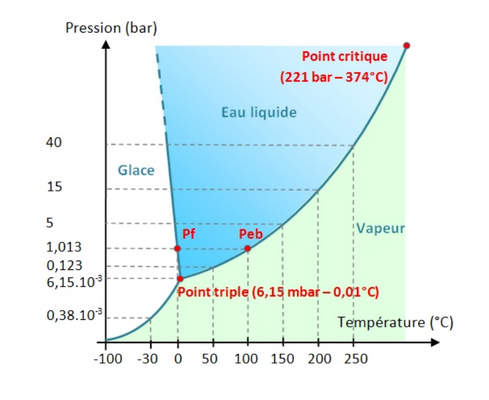
\includegraphics[scale = 0.55]{pT_water.png}
		\caption{Diagramme $(p,T)$ de l'eau. On insistera sur la pente de la frontière 
		liquide/solide, inhabituelle.}
	\end{center}
\end{figure}

\subsection{Variance}

L'état d'équilibre d'un système est décrit à l'aide de paramètres. On peut donc \textbf{obtenir un équilibre particulier en fixant des paramètres intensifs}. \textbf{Combien de paramètres faut-il fixer pour obtenir l'équilibre désiré ?} On peut le savoir en introduisant une nombre appelé variance.\\

La \textbf{variance est le nombre nécessaire et suffisant de paramètres intensifs indépendants que l'expérimentateur peut choisir pour fixer totalement l'état d'équilibre du système}. On traduit cette définition par la relation suivante :
\begin{equation}
	\boxed{V = X - Y}
\end{equation}
avec $X$ le nombre de paramètres intensifs (température, pression, composition) et $Y$ le nombre de relations entre eux à l'équilibre. Inversement en connaissant la valeur des v paramètres intensifs indépendants, on peut retrouver la valeur des X paramètres intensifs à partir des Y relations.\\

Appuyons-nous sur le diagramme de l'eau et calculons la variance dans plusieurs cas :
\begin{itemize}
%	\item si l'eau se trouve à l'équilibre dans une phase unique (par exemple liquide), on peut choisir librement température et pression sans modifier la nature de l'équilibre. Les variables intensives sont $P$, $T$ et $x^l(\text{H}_2\text{O})$, fraction molaire en eau de la phase liquide. On a une relation de contrainte :
%	\begin{equation}
%		x^l(\text{H}_2\text{O}) = 1, \quad\text{d'où}\quad V = 3 - 1 = 2.
%	\end{equation}
	\item si l'eau se trouve à l'équilibre dans une phase unique (par exemple liquide), on peut choisir librement température et pression sans modifier la nature de l'équilibre. Les variables intensives sont $P$ et $T$, sans relation entre elles :
	\begin{equation}
		V = 2 - 0 = 2.
	\end{equation}
	On peut ainsi choisir librement $T$ et $p$. En chauffant de manière isobare un solide ou un liquide, sa température augmente. Dans l'un des trois domaines figurant sur le diagramme, la phase stable est \textbf{celle dont le potentiel chimique est le plus faible sous les conditions considérées};\\
	
	\item si l'eau est en équilibre sous deux phases (solide-liquide par exemple), on ne peut plus choisir qu'un seul paramètre. Sur le diagramme cette transition correspond aux courbes. On voit alors qu'en fixant la pression, la température est fixée. Calculons la variance : les variables intensives sont $p$, $T$, $x^l(\text{H}_2\text{O})$, et $x^s(\text{H}_2\text{O})$ décrivant la composition des phases liquide et solide, sous-systèmes du corps pur. Les relations de contrainte sont au nombre de trois :
	\begin{equation}
		x^l(\text{H}_2\text{O}) = 1,\quad x^s(\text{H}_2\text{O}) = 1 
		\quad\text{et}\quad = \mu^{*,s}(T,p) = \mu^{*,l}(T,p),
	\end{equation}
	d'où la variance
	\begin{equation}
		V = 4 - 3 = 1.\quad\text{On ne peut plus choisir qu'un seul paramètre intensif.}
	\end{equation}
	Lorsqu'on chauffe de la glace sous 1 bar et qu'elle commence à fondre, on obtient un système à deux phases avec aucun degré de liberté (la pression étant déjà choisie par l'expérimentateur). Cela se traduit par la présence d'un palier de température : on chauffe le système mais sa température n'augmente plus tant qu'il reste la phase solide. La courbe obtenue en traçant $T = f(t)$ est appelée \textbf{courbe d'analyse thermique}. \textcolor{red}{Tracer et présenter la courbe de refroidissement de l'acide acétique glacial.};\\

	\item si l'eau est en \textbf{équilibre sous trois phases} on est en présence du \textbf{point triple}. Les variables intensives sont au nombre de 5 ($p$, $T$, $x(\text{H}_2\text{O}(l)$, 
$x(\text{H}_2\text{O}(g)$, $x(\text{H}_2\text{O}(s)$) et il y a 5 relations entre ces paramètres
	\begin{equation}
		x^l(\text{H}_2\text{O}) = 1,\quad x^g(\text{H}_2\text{O}) = 1,
		\quad x^s(\text{H}_2\text{O}) = 1
	\end{equation}
	ainsi que
	\begin{equation}
		\mu^{*,s}(T,p) = \mu^{*,l}(T,p)\quad\text{et}\quad \mu^{*,s}(T,p) = \mu^{*,g}(T,p),
	\end{equation}
	d'où la variance
	\begin{equation}
		V = 5 - 5 = 0.
	\end{equation}
	\textbf{Les conditions d'observation du point triple} sont fixées et \textbf{ne laissent pas de 		place au choix}, ni pour la pression, ni pour la température.
\end{itemize}

\section{Mélanges binaires liquide-solide}

Un mélange binaire est un mélange de deux corps purs supposés non réactifs entre eux, par exemple un alliage métallique (comme le bronze, alliage de cuivre et d'étain), ou l'électrum, un alliage précieux d'or et d'argent utilisé comme monnaie ou en décoration à l'Antiquité) ou encore de l'eau salée. On va s'intéresser exclusivement à des transformations isobares.

\subsection{Refroidissement isobare d'un mélange binaire}

On propose de suivre le refroidissement isobare d'un mélange acide acétique / eau : 10 mL d'acide pour 5 gouttes d'eau. \textcolor{red}{Manip : refroidissement en direct d'un mélange acide acétique glacial/eau pour illustrer la disparition du palier horizontal (lors du changement d'état). Comparaison avec la courbe de refroidissement du corps pur précédemment tracée. Pour bien voir la rupture de pente, elle doit se faire à une température suffisamment éloignée de celle du bain de glace fondante. Éventuellement montrer le résultat obtenu en préparation pour gagner du temps. Dire que la rupture de pente correspond à l'apparition du premier cristal solide.}

\subsection{Potentiel chimique d'un constituant dans un mélange}

On va généraliser la notion de potentiel chimique à un mélange de plusieurs constituants. Puisque $G$ est extensive 
\begin{equation}
	G(T,p,n_i) = \sum_{i = 1}^{N} n_i G_{m,i} = \sum_{i = 1}^{N} n_i \mu_i
	\quad\text{avec}\quad 
	\mu_i(T,p,\{x_j\}) = \left(\frac{\partial G}{\partial n_i}\right)_{T,p,n_j\neq n_i}.
\end{equation}

%Les relations de Maxwell introduites précédemment se généralisent à chaque constituant
%\begin{equation}
%	\left(\frac{\partial \mu_i}{\partial T}\right)_{p,x_j} = 
%	-\left(\frac{\partial S_{m,i}}{\partial n_i}\right)_{T,p,n_j\neq n_i} = -S_{m,i}
%	\quad\text{et}\quad 
%	\left(\frac{\partial \mu_i}{\partial p}\right)_{T,x_j}
%	= \left(\frac{\partial V}{\partial n_i}\right)_{T,p,n_j\neq n_i} = V_{m,i}. 	
%\end{equation}

Le potentiel chimique de l'espèce $i$ dans un mélange est une grandeur intensive, qui ne dépend que de la composition (en fraction molaire $x_j$ ou massique $w_j$ de chaque constituant), de la pression et de la température.\\

\textbf{Dans une phase $\phi$ donnée}, le potentiel chimique de l'espèce $i$ s'écrit
\begin{equation}
	\boxed{\mu_i^\phi(T,p,\text{comp}) = \mu_i^{\circ,\phi}(T)+ RT\text{ln}(a_i^\phi)} 
\end{equation}
avec $a_i^\Phi$ l'activité chimique de l'espèce $i$ dans la phase $\phi$. Dans le cas où on a un mélange idéal en phase liquide ou gazeuse,
\begin{equation}
	a_i^\phi = x_i^\phi.
\end{equation}

\subsection{Mélanges binaires homogènes}

On commence par supposer une \textbf{miscibilité totale des deux espèces en phase solide}, ces mélanges dits homogènes sont rares : les éléments doivent être voisins dans la classification périodique (même ligne, colonne voisine ou l'inverse), avoir des structures cristallines similaires et des rayons atomiques compatibles. Ceci ne garantit cependant pas un mélange idéal (ex : Au/Pt).

	\subsubsection{Mélange idéal : exemple des cupronickels}
	
	\textcolor{red}{Montrer un diagramme binaire :}
	\begin{itemize}
		\item Axes : température et fraction massique ou molaire en l'une des deux espèces;
		\item On note la température de fusion des corps purs;
		\item \textbf{\textcolor{red}{Obtention des diagrammes :}}
			\begin{itemize}
			\item la premier façon d'obtenir un tel diagramme est de tracer les courbes d'analyse 					thermique pour des compositions différentes. Leur allure est cependant différente de 					celle que l'on peut obtenir avec un corps pur;
			\item l'écriture des conditions d'équilibre en utilisant le potentiel chimique (hors 					programme) permet pour un mélange idéal de calculer des expressions pour les deux     	   			courbes présentes sur le diagramme : le \textbf{liquidus} et le \textbf{solidus};
			\item définir \textbf{solidus} (apparition du premier cristal en refroidissant) et 						\textbf{liquidus} (frontière liquide-diphasique). Discuter les phases en présence dans 					chaque zone; 
			\end{itemize}
		\item Tracer un modèle schématique de courbe de refroidissement sur un déplacement vertical, 		\textbf{\textcolor{red}{commenter la variance}} pour chaque section de la courbe.\\
		
		\item \textbf{\textcolor{red}{Expliquer comment lire un diagramme.}} Pour une composition 				totale du mélange, à une température donnée :
			\begin{itemize}
			\item l'intersection entre l'horizontale passant par le point ($x_B$,$T$) et le liquidus 				donne la composition en B de la phase liquide;
			\item l'intersection entre l'horizontale passant par le point ($x_B$,$T$) et le solidus 				donne la composition en B de la phase solide;
			\end{itemize}	
		\item \textbf{Règle des moments :}
			\begin{equation}
				n_B = x_B^l n^l + x_B^s n^s \quad\text{d'une part, et d'autre part}\quad
				n_B = x_B n = x_B (n^l + n^s) 
			\end{equation}
			d'où, en égalisant les deux expressions,
			\begin{equation}
				\boxed{\frac{n^l}{n^s} = \frac{x_B^s - x_B}{x_B - x_B^l}}.
			\end{equation}				
	\end{itemize}

	\subsubsection{Mélange non-idéal : point indifférent}
	Dans le cas d'un mélange non idéal, le fuseau peut être déformé. Dans certains cas, le diagramme présente deux fuseaux connectés par un point, c'est le \textbf{point indifférent}, de coordonnées $(x_I,T_I)$. Un mélange de composition globale $x_I$ changera d'état à température constante, tout comme un corps pur : phase liquide et phase solide auront la même composition. \textcolor{red}{Montrer le diagramme Vanadium-Titane : le vanadium améliore la ductilité du titane, c'est à dire sa capacité à s'étirer sans se rompre.}
		
\subsection{Mélanges inhomogènes}

\subsubsection{Non-miscibilité à l'état solide}
	
Cette situation est bien plus fréquente que la précédente. On va s'appuyer sur le mélange acide acétique eau.
\begin{itemize}
	\item présentation des domaines : liquide, liquide $+$ solide A, liquide $+$ solide B, 		solide A $+$ solide B;
	\item ligne eutectique $T^E$ : coexistence de trois phases, phase liquide de 					composition $x_E$, phase solide A pure et phase solide B pure;
	\item point eutectique $(x_E,T_E)$ : changement d'état type corps pur à 
		composition $x_E$ de la phase liquide constante;
	\item courbes de refroidissement en vis à vis du diagramme pour une verticale passant 			par le point E et par une verticale passant à côté. Lors du passage par la ligne 			eutectique, $T$ reste constante tant qu'il reste une goutte de liquide.
\end{itemize} 

Application au salage des routes en période hivernale : diagramme eau/chlorure de sodium. Nécessité de rouler sur la glace pour la faire fondre, pour que l'eau se mélange au sel, le mélange ayant un point de fusion plus bas que l'eau pure.

\subsubsection{Composés définis}

Apparition de phases solides nouvelles, de structure microscopique très différente de celle des corps purs pris individuellement : notion de composé défini. Pour illustrer, exemple du diagramme isobare Mg-Zn : remonter à la formule du composé défini et pointer la température de fusion du composé défini.\\

\section*{Conclusion}

Le potentiel chimique joue, en thermodynamique, un rôle similaire à la température et à la pression en cela qu'une différence de potentiel entre deux sous systèmes implique un transfert de matière du sous-système de potentiel le plus grand vers celui de potentiel le plus faible. C'est un outil précieux qui permet d'étudier les systèmes ouverts, ou les systèmes fermés dont la composition interne varie. Nous avons utilisé cette notion dans le cadre de l'étude du changement d'état du corps pur et des mélanges binaires.\\

Le changement d'état d'un mélange binaire diffère de celui d'un corps pur. Les diagrammes binaires, construits empiriquement par analyse des courbes de refroidissement représentent de façon synthétique un grand nombre d'information, par exemple l'existence et la composition des phases pour une température $T$ et une pression $p$ donnée.\\

Ouverture vers l'utilisation du potentiel chimique pour l'étude thermodynamique des réactions chimiques : prévision du sens d'évolution et de la composition à l'équilibre.

\newpage
\section*{Annexes}
\subsection{Protocole d'obtention des courbes de refroidissement}
\begin{itemize}
	\item Nettoyer la verrerie à l'acétone (pas à l'eau pour éviter qu'elle ne se mélange à 				l'acide), sécher à l'air comprimé.
	\item Sous la hotte, introduire 10 mL d'acide dans un tube à essai à 25$\degree$C, thermostaté 			dans un bécher d'eau chaude.
	\item Mettre de la glace fondante dans le Dewar.
	\item Plonger touillette et thermomètre dans le tube à essai.
	\item Plonger le tout dans le Dewar.
	\item Lancer l'acquisition, repérer le palier de température.	
\end{itemize}

\subsubsection*{Remarques}
\begin{itemize}
	\item touiller légèrement pour éviter la surfusion,
	\item impossible de trouver l'eutectique, température trop faible !
	\item travailler avec de faibles quantités d'eau (5 gouttes pour 10 mL maximum)
\end{itemize}
\end{document}